\documentclass[parskip=full]{scrartcl}
\usepackage[T1]{fontenc}
\usepackage[utf8]{inputenc}
\usepackage[ngerman]{babel}
\usepackage{hyperref}
\hypersetup{
pdftitle={PSE: Blockchain-basiertes E-Voting - Entwurfsdokument},%
,%
}
\usepackage{graphicx}
\usepackage{csquotes}
\usepackage[nonumberlist]{glossaries}
\usepackage{enumitem}
\usepackage{xcolor}
\usepackage{rotating}
\usepackage{svg}
\usepackage[section]{placeins}
\makeatletter
\AtBeginDocument{%
	\expandafter\renewcommand\expandafter\subsection\expandafter{%
		\expandafter\@fb@secFB\subsection
	}%
}
\makeatother
\makeatletter
\AtBeginDocument{%
	\expandafter\renewcommand\expandafter\subsubsection\expandafter{%
		\expandafter\@fb@secFB\subsubsection
	}%
}
\makeatother

\addto\extrasngerman{\def\figureautorefname{Abb.}}
\newcommand{\textitx}[1]{\mbox{\textit{#1}}}
\newcommand{\fakeparagraph}[1]{\textbf{#1}}
\renewcommand{\includesvg}[1][1]{}

\title{PSE: Blockchain-basiertes E-Voting}
\author{Tim Fröhlich, Achim Kriso, Philipp Schaback, David Schuldes, Artem Vasilev\\ Phasenverantwortlicher: David Schuldes}

\begin{document}
	\clearpage
	\maketitle
	\pagenumbering{gobble}
	\newpage
	
	\tableofcontents
	\newpage
	\pagenumbering{arabic}
	\section{Einleitung}
	Dieses Dokument beschreibt die Ergebnisse der Entwurfsphase im Rahmen des Moduls Praxis der Softwareentwicklung (PSE) am Karlsruher Institut für Technologie, das am Lehrstuhl für Anwendungsorientierte formale Verifikation von Professor Beckert ausgeschrieben wurde.
	Entworfen wurde die im Pflichtenheft definierte Software "Blockchain-basiertes E-voting". 
	
	Ziel der Software ist es, die Manipulation
	von Wahlergebnissen zu verhindern und den Wählern zu gewährleisten, dass ihre Stimme unverändert in die Wahl eingegangen ist.
	Ziel dieses Dokumentes ist es, zu erläutern wie die im Pflichtenheft spezifizierten Anforderungen softwaretechnisch umgesetzt werden sollen.
	
	\section{Architektur}
	\begin{figure}[!h]
	\centering
	\includesvg[width=\textwidth]{pictures/PackageDiagram.svg}
	\caption{Übersicht der Pakete und deren Interaktion}
	\end{figure}

	Basierend auf der Model-View-Control Architektur ist die Software in ein Model-Paket, View-Paket und Control-Paket unterteilt und jede Assoziation zwischen den Paketen durch eine Schnittstelle klar definiert. 
	\\
	Die Entwurfs-Architektur hat zwei Klienten, einen Wahlleiter- und einen Wähler-Klient. Die Schnittstellen, die von beiden Klienten nach außen angeboten werden, bestehen aus einer Hierarchie von drei Interfaces. Ein Interface welches die Gemeinsamkeiten der beiden Klienten erfasst und jeweils ein Interface für jeden Klienten der das allgemeine Interface um die benötigte Funktionalität erweitert. Dabei spiegelt der Name eines Interfaces eine unidirektionale Assoziation zwischen den Paketen die es repräsentiert wider. Beispielsweise ist \textitx{ControlToViewIF} das Interface ,welches das Control-Paket benutzt um auf Funktionalität des View-Pakets zuzugreifen.
	\\
	Das \textitx{ElectionDataIF} dient als Data Transfer Object. Es bietet alle Getter-Methoden, um auf die allgemeinen Daten einer Wahl zuzugreifen. Dieses Interface wird von den Paketen implementiert, die von Rohdaten (Beispielsweise aus der Blockchain) eine Wahl laden. Es ist dann möglich ohne Probleme dieses Objekt an andere Pakete zu übertragen, ohne die Modularität des Entwurfs zu verletzen.
	\\
	Das View- und Control-Paket stehen in einer bidirektionalen Assoziation zueinander. Beide Pakete haben außerdem eine Unidirektionale Assoziation zu dem Model-Paket. Die einzige Ausnahme zu diesem System an Schnittstellen ist der Callback-Listener \textit{ElectionStatusListener}, der von dem Model benutzt wird um das View-Paket bei Wahlende zu benachrichtigen und von dem Blockchain-Netzwerk ausgeht.
	\\
	\begin{itemize}
		\item[View:] Dieses Paket dient zur Darstellung der Benutzeroberfläche und benutzt das Java Swing GUI Framework für die Darstellung der einzelnen GUI Elemente. Außerdem enthält das Paket eine Reihe an eigenen Elementen, die für speziellere Anforderungen dieses Projektes konstruiert wurden. Unterschiede zwischen den beiden Klienten finden sich vor allem in der Darstellung der Benutzeroberflächen, deswegen sind sie in zwei Unterpakete unterteilt.
		\item[Control:] Der Controller nutzt die vom Java Swing Framework gebotenen Listener, die vom Control-Paket an das View-Paket weitergeleitet werden, um direkt auf Benutzereingaben einzugehen. Sobald Control eine Eingabe empfängt werden Aufgaben abhängig davon welcher Listener ausgelöst wurde über die Schnittstellen an das Model oder View Paket weitergeleitet. Wie das View Paket ist auch das Control Paket in ein Subpaket für den Wahlleiter und ein Subpaket für den Wähler unterteilt. Die Subpakete enthalten jeweils eine spezielle Implementierung des \textitx{ViewToControl} Interfaces und alle benötigten Listener.
		\item[Model:] Das Model-Paket hat zwei Hauptaufgaben. Es verwaltet alle zustandsrelevanten Daten und hält die Schnittstelle zu dem Blockchain-Netzwerk über die vom Hyperledger Framework gebotenen Schnittstellen. Diese zwei Aufgaben sind in zwei Subpakete unterteilt. Das SDKConnection Paket, welches die Schnittstellen des Hyperledger Frameworks auf die Anforderungen der Software anpasst, und das StateManagement Paket welches alle Daten bereitstellt und deren interne Logik enthält.   
	\end{itemize} 
\subsection{Interfaces zwischen den Paketen}
	\begin{itemize}
	\item\fakeparagraph{ViewToModelIF} Das ViewToModelIF bietet der View ein Interface um auf die Datenhaltung zuzugreifen.
	Es werden Methoden bereitgestellt, die es ermöglichen allgemeine Daten zur Wahl abzufragen.
	Die hiervon ausgehenden konkreten Interfaces SupervisorViewToModelIF und VoterViewToModelIF stellen zusätzlich Methoden zur Verfügung. Diese fragen Daten ab, die lediglich für den Wahlleiter oder respektive nur für den Wähler relevant sind.
	Die Methode setElectionEndListener dient dem Festlegen eines ActionListeners für das Wahlende beim initialen starten des Programms.
	\end{itemize} 

	\begin{itemize}
	\item\fakeparagraph{ControlToModelIF} Das ControlToModelIF bietet der Control ein Interface um auf die Datenhaltung zuzugreifen.
	Es werden Methoden bereitgestellt, die es ermöglichen die Daten auf der Datenhaltung zu manipulieren und entsprechende Zugriffe auf das Blockchain Netzwerk auszuführen.
	Die hiervon ausgehenden konkreten Interfaces VoterControlToModelIF und SupervisorControlToModelIF stellen zusätzlich Methoden zur Verfügung. Diese ermöglichen Netzwerkzugriffe und Datenmanipulation, die lediglich für den Wahlleiter oder respektive nur für den Wähler relevant oder erlaubt sind.
	Diese Interfaces erfüllen mitunter \textbf{F1, F2, F3, F4, F5, F6, F7, F8, F9, F10} aus Sicht des View-Pakets.
	\end{itemize} 

	\begin{itemize}
	\item\fakeparagraph{ControlToViewIF} Das ControlToViewIF bietet der Control ein Interface um auf die GUI zuzugreifen.
	Die hiervon ausgehenden konkreten Interfaces VoterControlToViewIF und SupervisorControlToViewIF stellen zusätzlich Methoden zur Verfügung, die nur für den Wahlleiter oder respektive nur für den Wähler relevant sind. 
	Diese Gruppe von Interfaces erfüllen Hauptsächlich zwei Funktionen: Manipulation der GUI bei relevanten Änderungen im System und dem Abfragen von ausgefüllten Daten an der GUI.
	Diese Interfaces ermöglichen zudem das Übermitteln von Fehler- oder Erfolgsmeldungen an die GUI.
	Diese Interfaces erfüllen mitunter \textbf{F1, F11, F13} aus Perspektive des View-Pakets.
	\end{itemize} 
	\begin{itemize}
	\item\fakeparagraph{ControlToViewIF} Das ControlToViewIF bietet der Control ein Interface um auf die GUI zuzugreifen.
	Die hiervon ausgehenden konkreten Interfaces VoterControlToViewIF und SupervisorControlToViewIF stellen zusätzlich Methoden zur Verfügung, die nur für den Wahlleiter oder respektive nur für den Wähler relevant sind. 
	Diese Gruppe von Interfaces erfüllen Hauptsächlich zwei Funktionen: Manipulation der GUI bei relevanten Änderungen im System und dem Abfragen von ausgefüllten Daten an der GUI.
	Diese Interfaces ermöglichen zudem das Übermitteln von Fehler- oder Erfolgsmeldungen an die GUI.
	Diese Interfaces sorgen mitunter für die Erfüllung von \textbf{F1, F11, F13}.
	\end{itemize} 
	\begin{itemize}
	\item\fakeparagraph{ViewToControlIF} Das ViewToControlIF und seine Subklassen dienen ledigglich dem Weiterleiten aller Notwendigen ActionListener an die GUI, damit diese dort an entsprechenden Komponenten registriert werden können.
	\end{itemize} 
	\begin{itemize}
	\item\fakeparagraph{ElectionStatusListener} Das ElectionStatusListener Interface bietet dem Model möglichkeiten der GUI den Status der Wahl mitzuteilen. So kann ein update der Daten angefragt werden oder die Beendigung der Wahl mittgeteilt werden.
	Dieser Listener sorgt mitunter für die Erfüllung von \textbf{F14, F15}.
	\end{itemize} 
  
	\subsection{Typische Abläufe}
	\begin{itemize}
	\item\fakeparagraph{Aufbau der Topologie, \autoref{fig:main_thread} } Beim initialen starten der Anwendung (Hier aus Sicht des Wahlleiters), wird zuerst die SupervisorGUI Klasse erstellt. Daraufhin wir der Listener für den Status der Wahl erstellt. Danach wird das Model aufgebaut und der erstellte listener registriert. Danach wird die Control erstellt und das Model dort registriert. Im Anschluss wird der Supervisor Adapter erstellt und die Control an diesem registriert. Letztlich wird der Anzuzeigende Panel erstellt und somit die Benutzeroberfläche angezeigt.
	Der Aufbau der Topologie aus Sicht des Wählers geschieht analog.
	Initialisierung der SDK Schnittstelle und deren Topologie erfolgt an dieser Stelle noch nicht, dies geschieht bei der ersten Authentifizierung.
	
	\item\fakeparagraph{Import einer Wahlkonfiguration, \autoref{fig:config_import}} Nach Auslösen des ImportConfigListeners, wird in der View nach dem ausgewählten Pfad gefragt. Dieser Pfad wird an das Model gegeben, welches die Datei liest und dort die abgespeicherten Daten in ihren Attributen ablegt.
	Schließlich wird die View vom ImportConfigListener dazu aufgefordert die Daten aus dem Model zu holen und in ihrer ConfigGUI anzuzeigen.
	Dabei holt die SupervisorGUI die Wahldaten als ein ElectionDataIF Data-Transfer-Object und die, in der Konfiguration definierten Wähler. Diese beiden Daten Objekte werden dann einzeln an die ConfigGUI gereicht, welche die im ElectionDataIF enthaltenen Daten extrahiert und in den entsprechenden SupervisorGUIPanel Objekten einsetzt.
	
	\item\fakeparagraph{Authentifizierung, \autoref{fig:voter_auth} } Zuerst drückt der Wähler den Knopf "Weiter", daraufhin wird actionPerformed() aufgerufen.
	Dann beginnt die Autorisierung durch den Aufruf von authorization() auf einem VoterElection Objekt.
	Durch getAuthentication() wird der angegebene Pfad aus der GUI gelesen.
	Daraufhin wird eine VoterSDKInterfaceImpl instanziiert und erhält zwei Parameter: Den Pfad zum Wähler-Zertifikat und einen Listener.
	Mit der start Methode wird ein neuer Thread der SDKEventListenerImpl erzeugt, welcher regelmäßig den Status der Wahl aus dem Netzwerk abfragt.
	Bei erfolgreich abgeschlossener Authentifizierung wird durch showChoice() auf der VoterGUI eine neues VoterChoice Panel erstellt und angezeigt, welches die Ansicht ist auf der es dem Wähler möglich ist zu wählen.
	
	\item\fakeparagraph{Wahl, \autoref{fig:vote_sequence} } Bei betätigen des Wahl buttons durch den Wähler wird der ActionListener "VotedListener", welcher im Controller package liegt aufgerufen. Dieser holt sich daraufhin die vom Wähler getroffene Auswahl aus dem GUI package mittels dem ControllerToViewIF. Im Anschluss wird die getroffene Wahl an das Model weitergegeben, wo dann die Wahl an das Netzwerk weitergegeben wird. Bei erfolgreichem Speichern der Wahl im Blockchain-Netzwerk wird diese auch in der Datenhaltung so übernommen. Zuletzt führt der VotedListener bei erfolgreich abgegebener Stimme die showWaiting Methode auf der GUI auf, welche dafür sorgt, dass die Ansicht zwischen Wahlabgabe und Wahlende für den Wähler angezeigt wird. Hierfür wird eine neue Instanz der VoterWait Klasse erstellt, welche sich zuerst über den VoterAdapter die Notwendigen Daten holt und daraufhin mithilfe des VoterMajorityVotingSystemComponentManager die Notwendigen GUI Komponenten zusammenstellt und anzeigt.
	
	\end{itemize}
	\newpage
	\pagestyle{empty}
		\begin{sidewaysfigure}[!h]
		\centering
		\hspace{-100pt}
		\centerline{\includesvg[width=1.3\textwidth]{pictures/MainThreadSequenceDiagram}}
		\caption{Start der Anwendung, Aufbau der Topologie}
		\label{fig:main_thread}
	\end{sidewaysfigure}

	\newpage
	\begin{sidewaysfigure}[!h]
		\centering
		\hspace{-100pt}
		\centerline{\includesvg[width=1.3\textwidth]{pictures/ImportConfig}}
		\caption{Importieren einer Wahlkonfiguration}
		\label{fig:config_import}
	\end{sidewaysfigure}

	\newpage
	\begin{sidewaysfigure}[!h]
		\centering
		\hspace{-100pt}
		\centerline{\includesvg[width=1.3\textwidth]{pictures/VoterAuthenticationSequenceDiagram}}
		\caption{Authentifizierung eines Wählers gegenüber des Netzwerks}
		\label{fig:voter_auth}
	\end{sidewaysfigure}

	\newpage
	\begin{sidewaysfigure}[!h]
		\centering
		\hspace{-100pt}
		\centerline{\includesvg[width=1.3\textwidth]{pictures/VoteSequenceDiagram}}
		\caption{Abgabe einer Stimme durch einen Wähler}
		\label{fig:vote_sequence}
	\end{sidewaysfigure}

	\newpage
	\section{Model}
	\pagestyle{plain}
	Die zwei Subpakete in Model kommunizieren über die definierte Schnittstelle \textitx{SDKInterface} und einen Callback Listener \textitx{SDKEventListener}. 
	Damit der Klient darüber informiert ist, ob die Wahl noch läuft wird der \textitx{SDKEventListener} benutzt. Ein Klient kann über die Schnittstellenmethode \textitx{dispatchElectionOverCheck()} eine Überprüfung auf der Blockchain Anforderung, die herausfindet ob die Wahl geendet hat. Wenn das der Fall ist wird der die Methode \textitx{onElectionEnd()} in jedem Klienten aufgerufen. Wenn die Wahl noch nicht zuende ist wird \textitx{onElectionRunning()} in jedem Klienten aufgerufen. Dieses System wird benutzt um unnötige \textitx{dispatchElectionOverCheck()} Aufrufe zu vermeiden. Jeder Klient überprüft, mithilfe eines Threads, wann das letzte mal \textitx{onElectionRunning()} aufgerufen wurde. Wenn dies Länger als die backoff Zeit in Minuten her ist, ruft der Klient selber \textitx{dispatchElectionOverCheck()} auf. Um zu verhindern das alle Klienten zum gleichen Zeitpunkt \textitx{dispatchElectionOverCheck()} aufrufen, wird die backoff Zeit in jedem Klienten zufällig in in einem Zeitraum gewählt. Sobald einmal \textitx{onElectionOver()} aufgerufen wurde, muss der Thread nie wieder \textitx{dispatchElectionOverCheck()} aufrufen und er setzt \textitx{hasEnded} auf wahr und beendet sich.
	Die Schnittstelle ist wieder in drei Interfaces unterteilt. Eine für die Gemeinsamkeiten (\textitx{SDKInterface}) der beiden Klienten und jeweils eine für die Unterschiede (\textitx{SupervisorSDKInterface} und \textitx{VoterSDKInterface}).

	\subsection{Paket: StateManagement}
	Das StateManagement Paket hat die Aufgabe alle wichtigen Zustandsdaten zu speichern, für die View zugänglich und die Logik der Daten zu implementieren.
	Dabei kommuniziert es mit dem SDKConnection Paket um Daten von der Blockchain zu holen und Aktionen auf der Blockchain auszuführen.
	
		\subsubsection{Election}
		Im Zentrum dieses Paketes ist die \textitx{Election} Klasse. Sie speichert die Kandidaten, Stimmen und Allgemeine Wahldaten in Form des \textitx{ElectionDataIF}. Außerdem hält es den SDKEventListener um über den Zustand der, auf 
		der Blockchain, laufenden Wahl informiert zu werden.\\
		Die \textitx{Election} Klasse wird erweitert durch ...
		\begin{itemize}
			\item\fakeparagraph{SupervisorElection} um die nötige Funktionalität für den Wahlleiter hinzuzufügen. Dies beeinhaltet alle Wähler und eine Assoziation zu \textitx{SupervisorSDKInterface}.
			\item\fakeparagraph{VoterElection} in der der Wähler seine eigene Stimme speichert und eine Assoziation zu \textitx{VoterSDKInterface} hat.
		\end{itemize}
		
		\subsubsection{VotingSystem}
		Das Verhalten des Systems ist abhängig davon, welches Auszählverfahren für die Wahl festgelegt wird. Im StateManagement Paket wird bestimmt welche Art der Stimmabgabe benutzt wird und wie der Gewinner ermittelt wird.
		Um diese Funktionen objekt-orientiert zu entwerfen existiert die abstrakte Klasse \textitx{VotingSystem}. Sie setzt voraus, dass alle Implementationen eine \textitx{loadVote(vote : String)}-Methode und \textitx{determineWinner()}-Methode implementieren. Die \textitx{loadVote(vote : String)}-Methode dient dazu, Stimmen die in Form eines String vorliegen in Vote-Objekte umzuwandeln. \textitx{determineWinner()} evaluiert alle gespeicherten Stimme in dem \textitx{Election} Objekt und bestimmt, welcher Kandidat gewonnen hat. Damit wird \textbf{F15: Auszählung der Stimmen} erfüllt.
		Da beim Start eines Klienten das Wahlsystem nur als String vorliegt (entweder von der Blockchain geladen oder in der Konfigurationbenutzeroberläche eingegeben), wird die Klasse \textit{VotingSystemBuilder} benutzt um diesen String in ein \textitx{VotingSystem} Objekt konvertieren.
		Zur Vereinfachung der Implementation von \textitx{VotingSystem} haben \textitx{Vote}-Klassen eine \textitx{asString()}-Methode welche ihren Zustand in einen String umwandeln. Solche Strings können durch die statische Methode \textitx{loadVote(vote : String)} wieder in ein äquivalentes Vote-Objekt umgewandelt werden. Der Aufbau eines solchen Strings ist abhängig vom gewählten VotingSystem. Hier wird eine Serialisierung des entsprechenden Vote-Objektes zu einem JSON-String vorgenommen, welcher vom VotingSystem selbst wieder deserialisiert werden kann. Die Übertragung der Votes von View über den Control zum Model erfolgt ebenfalls in selbigem JSON-String Format.
	
	\subsection{Paket: SDKConnection}
	\subsubsection{Übersicht}
	Das Paket \textitx{SDKConnection} stellt die Verbindung der Software zum \textitx{Hyperledger Fabric SDK} und \textitx{Hyperledger Fabric CA SDK} dar. Diese SDKs übernehmen ihrerseits die Kommunikation mit dem Netzwerk. \textitx{SDKConnection} ist Teil des \textitx{Models}.
	\subsubsection{Wichtige Elemente der SDKConnection}
	\paragraph{SDKInterfaceImpl} ist eine Implementierung der generische Schnittstelle \textitx{SDKInterface}. Sie wird erweitert durch die klientspezifischen Implementierungen \textit{SupervisorSDKInterfaceImpl} und \textit{VoterSDKInterfaceImpl}. Sie bietet Zugriff auf die von beiden Klienten gemeinsam genutzen Funktionen, beispielsweise zur Popularisierung der Benutzeroberfläche mit Wahlinformationen nach einem Neustart derselbigen.
	\paragraph{SupervisorSDKInterfaceImpl} ist eine Implementierung der Schnittstelle \textit{SupervisorSDKInterface}. Sie bietet die zum Wahlleiter-Klienten spezifische Kommunikation mit dem SDK zum Erstellen und endgültigen Beenden der Wahl. Außerdem ermöglicht sie das Auslesen aller bisherigen Stimmen aus dem Ledger und das Erstellen neuer Benutzer.
	\paragraph{VoterSDKInterfaceImpl} ist eine Implementierung der Schnittstelle \textit{VoterSDKInterface}. Sie bietet die zum Wähler-Klienten spezifische Kommunikation mit dem SDK zum Abgeben einer Stimme und Auslesen der eigenen Stimme aus dem Ledger.
	\paragraph{AppUser} repräsentiert eine Person aus der Sicht des SDKs. Die Klasse realisiert die Schnittstellen \textitx{User} des Hyperledger SDKs und \textitx{Serializable} des Java SDKs. \textit{SupervisorSDKInterfaceImpl} erstellt Objekte dieses Typs und serialisiert sie zur Weitergabe an die Wähler.
	\paragraph{Transactions} beinhaltet die verschiedenen Transaktionen die mittels des SDKs zum Netzwerk gesendet werden können. Die in den Schnittstellen gebotenen Methoden benutzen jeweils eine dieser Klassen, um die entsprechende Transaktion zu kapseln. Die abstrakte Klasse \textit{Transaction} bietet die Schablonenmethode \textit{getFunctionName}, deren Implementierungen den Funktionsnamen der gegenstelligen Funktion im Chaincode zurückgeben. Dieser ist Teil jeder Anfrage an die Peers. Die Transaktionen werden grundsätzlich in zwei Kategorien aufgeteilt:
	\begin{enumerate}
			\item\fakeparagraph{QueryTransaction}: Transaktionen, die nur Daten anfragen, aber keine Änderungen am Datenbestand des Ledgers vornehmen. Bietet die Schablonenmethode \textit{parseResultString} deren Implementierungen das Parsen der Rückgabe übernehmen.
			\begin{itemize}
				\item \fakeparagraph{MultiStringTypeQuery}: Implementiert \textit{parseResultString} für Anfragen deren Rückgabe als mehrere Strings zu interpretieren ist.
				\subitem \fakeparagraph{AllVotesQuery}: Gibt alle Stimmen zur Auswertung zurück.
				\item \fakeparagraph{SingleStringTypeQuery}: Implementiert \textit{parseResultString} für Anfragen deren Rückgabe als ein einzelner String zu interpretieren ist.
				\subitem \fakeparagraph{OwnVoteQuery}: Gibt die Stimme des \textitx{AppUsers} zurück.
				\item \fakeparagraph{ElectionDataTypeQuery}: Implementiert \textit{parseResultString} für Anfragen deren Rückgabe als \textit{ElectionData} zu interpretieren ist.
				\subitem \fakeparagraph{ElectionDataQuery}: Gibt alle Metadaten der Wahl zurück.
			\end{itemize}
			\item \fakeparagraph{InvokeTransaction}: Transaktionen, die Änderungen am Datenbestand des Ledgers vornehmen, aber keine Daten zurückgeben. Die Konstruktoren dieser Klassen wandeln die übergeben Parameter in ein JSON-String um, welcher dann in \textitx{InvokeTransaction.invoke()} an das SDK übergeben wird.
			\begin{itemize}
				\item \fakeparagraph{VoteInvocation}: Gibt die Stimme des \textitx{AppUsers} ab.
				\item \fakeparagraph{InitializationInvocation}: Initialisiert die Wahl auf dem Ledger
				\item \fakeparagraph{ElectionStatusUpdateInvocation}: Löst ein Update-Event im Chaincode aus, welches von allen \textitx{ElectionStatusListenern} empfangen wird.
				\item \fakeparagraph{DestructionInvocation}: Startet das Netzwerk neu, um die Wahl endgültig zu beenden.
			\end{itemize}
	\end{enumerate}
	\newpage
	\begin{sidewaysfigure}[!h]
		\centering
		\hspace{-100pt}
		\centerline{\includesvg[width=1.3\textwidth]{pictures/Transactions}}
		\caption{Das Transactions-Paket}
		\label{fig:sdk_transaction}
	\end{sidewaysfigure}
	\thispagestyle{empty}
	\subsubsection{Typische Abläufe aus Sicht von SDKConnection}
	Im Nachfolgenden sollen die Teile der im Pflichtenheft beschrieben Testfallszenarien beschrieben werden, welche SDKConnection betreffen. Sie erfüllen außerdem die funktionalen Anforderungen \textbf{F1, F2, F3, F4, F6, F8, F16} aus Sicht von \textit{SDKConnection}.
	\\ \\ 
	% Nennung der Anforderungen beibehalten?
	Zuallererst registriert sich der Wahlleiter im Netzwerk (siehe \autoref{fig:sdk_first_registration}). Dazu erstellt das StateManagement eine Instanz von \textit{SupervisorSDKInterfaceImpl} und übermittelt dieser den Bootstrap-Username und das Bootstrap-Passwort. Diese wiederum erstellt eine Instanz von \textit{HFCAClient}, der Hyperledger Fabric CA Schnittstelle, um die Identität des Wahlleiters (Admins, aus der Sicht des SDKs) zu registrieren. Mit dieser Identität (\textit{Enrollment}) wird ein AppUser erstellt, welcher serialisiert und im mitgegebenen Dateipfad abgespeichert wird.
	\\ \\
	Als nächstes fügt das StateManagement die Wähler hinzu (siehe \autoref{fig:sdk_adding_voters}). Dazu ruft es die Methode \textit{createUser} für jeden User auf, welche einen \textit{RegistrationRequest} anlegt und mit diesem eine Identität beim \textit{HFCAClient} registriert. Der damit gebaute \textit{AppUser} wird serialisiert an den übergebenen Dateipfad geschrieben. Diese Dateien sind die Zertifikate, die an die Wähler verteilt werden müssen.
	\\ \\
	Dann werden die Wahldaten (\textit{ElectionDataInterface}) festgelegt, hierzu dient die Methode \textit{createElection} (siehe \autoref{fig:sdk_creating_election}). Diese erstellt die entsprechende Transaktion aus dem Transaction-Paket, \textit{InitializationInvocation}, welche wiederum die übermittelten Wahldaten in einen JSON-String verpackt. Mit der Methode \textit{invoke} wird die Transaktion ans SDK und von diesem an das Netzwerk gesendet.
	Damit ist das Erstellen einer Wahl aus der Sicht von \textit{SDKConnection} abgeschlossen. 
	\\ \\
	Aus der Sicht des Wählers läuft die Registrierung im Netzwerk ähnlich: Das StateManagement erstellt eine Instanz von \textit{VoterSDKInterfaceImpl} und übermittelt den Dateipfad zur vom Wahlleiter erhaltenen, serialisierten \textit{AppUser}-Klasse. Als nächstes fordert das StateManagement die Daten der Wahl an. Dies geschieht über die Methode \textit{getElectionData}.
	\\ \\
	Gibt der Wähler seine Stimme ab, so ruft das StateManagement \textit{vote} auf (siehe \autoref{fig:sdk_vote}). Analog zu \autoref{fig:sdk_creating_election} wird auch hier eine Instanz des richtigen Typs aus dem Transaction-Paket erstellt, von welchem auch hier die Parameter in einen JSON-String gewandelt und als \textit{TransactionProposalRequest} an das SDK gesendet werden.
	\\ \\	
	Zur Auswertung der Wahl ruft das StateManagement für den Wahlleiter die Methode \textit{getAllVotes} auf (siehe \autoref{fig:sdk_getallvotes}). Diese erstellt die entsprechende Transaktion \textit{AllVotesQuery},
	welche mit der Methode \textit{query} ans SDK und von diesem an das Netzwerk gesendet wird. Das Resultat der Anfrage wird als JSON-String empfangen, entpackt und an das StateManagement zurückgegeben. 
	\newpage
	\pagestyle{empty}
	\begin{sidewaysfigure}[!h]
		\centering
		\hspace{-100pt}
		\centerline{\includesvg[width=1.3\textwidth]{pictures/Authentication}}
		\caption{Erste Anmeldung des Wahlleiters im Netzwerk}
		\label{fig:sdk_first_registration}
	\end{sidewaysfigure}
	\newpage
	\begin{sidewaysfigure}[!h]
		\centering
		\hspace{-100pt}
		\centerline{\includesvg[width=1.3\textwidth]{pictures/AddingUsers}}
		\caption{Hinzufügen von neuen Wählern durch den Wahlleiter}
		\label{fig:sdk_adding_voters}
	\end{sidewaysfigure}
	\newpage
	\begin{sidewaysfigure}[!h]
		\centering
		\hspace{-100pt}
		\centerline{\includesvg[width=1.3\textwidth]{pictures/CreatingElection}}
		\caption{Erstellen einer Wahl durch den Wahlleiter}
		\label{fig:sdk_creating_election}
	\end{sidewaysfigure}
	\newpage
	\begin{sidewaysfigure}[!h]
		\centering
		\hspace{-100pt}
		\centerline{\includesvg[width=1.3\textwidth]{pictures/Vote}}
		\caption{Abgabe einer Stimme durch den Wähler}
		\label{fig:sdk_vote}
	\end{sidewaysfigure}
	\newpage
	\begin{sidewaysfigure}[!h]
		\centering
		\hspace{-100pt}
		\centerline{\includesvg[width=1.3\textwidth]{pictures/GetAllVotes}}
		\caption{Auslesen aller Stimmen durch den Wahlleiter}
		\label{fig:sdk_getallvotes}
	\end{sidewaysfigure}
	\newpage

	\section{View}
	\pagestyle{plain}	
		\subsection{Components}
		Dieses Unterpaket stellt dem Rest des View-Paketes Diagramme und ein modulares Tabellen-System bereit.
		
		\subsubsection{Diagramme}
		\begin{figure}[!h]
			\centering
			\includesvg[width=\textwidth]{pictures/DiagramClassDiagram.svg}
			\caption{Klassendiagram der Diagramme}
		\end{figure}
		
		Diagramme werden vom View-Paket benötigt, um die Ergebnisse einer Wahl in einer benutzerfreundlichen Form darzustellen. Für die unterstützten Wahlsysteme sind unterschiedliche Formen der Visualisierung sinnvoll. Deswegen wird eine allgemeine Diagramm-Schnittstelle geboten. Damit kann das Diagramm die benötigten Daten entgegennehmen und durch die Java Swing Graphics Schnittstelle, die in der Schablonenmethode \textitx{drawChart(g : Graphics)} überreicht wird, zeichnen. Es ist jeder Implementation dieser Schnittstelle überlassen, wie diese Daten zu interpretieren sind. Um die im Pflichtenheft beschriebenen Wahlsysteme zu unterstützen, existieren die Implementationen \textitx{PieChart} für die Mehrheitswahlsysteme und \textitx{StackedBarChart} für Instant Runoff Voting.
		
		\subsubsection{Tabellen}
		\begin{figure}[!h]
		\centering
		\includesvg[width=\textwidth]{pictures/ListExtensionClassDiagram.svg}
		\caption{Klassendiagram des Tabellensystems}
		\end{figure}
		
		Tabellen mit unterschiedlicher Struktur und Funktionalität werden in verschieden Bereichen der View benötigt (beispielsweise Wahlkonfiguration, Stimmabgabe und Ergebniseinsicht). Um redundanten UI Quellcode zu vermeiden wurde eine erweiterbare Tabelle entworfen, welche aus Verschiedenen Modulen (Erweiterungen) besteht mit denen sich alle bestehenden Anforderungen dieses Projektes erfüllen lassen.
		\\
		Grundlage ist eine Liste von Einträgen. Jeder Eintrag besteht aus den gleichen Komponenten. Ein Eintrag ist durch die Klasse \textitx{Entry} modelliert. Die Klasse \textitx{BasicList} implementiert das grundlegende Verhalten einer Liste. Dieses erfasst die Möglichkeit, durch die Tabelle zu scrollen, wenn sie nicht ganz in ihren Bereich passt und bietet die normale Schnittstelle einer jeden anderen Java Swing Komponente damit sie von dem Framework ohne Schwierigkeiten in die GUI integriert werden kann.
		\\
		Die Modularität dieses Tabellen Systems wird durch die Klasse \textitx{ExtendableList} implementiert. Diese Klasse ist eine Erweiterung von \textitx{BasicList}. Objekte die eine Instanz von \textitx{ListExtension} sind können durch den Konstruktor von \textitx{ExtendableList} zu der Tabelle hinzugefügt werden. Erweiterungen sind mithilfe des Dekorierer Entwurfsmusters umgesetzt. Sie werden miteinander verknüpft, indem jede Erweiterung eine andere durch ihren Konstruktor bekommen kann. Diese Kette an Erweiterungen wird schließlich dem Konstruktor der \textitx{ExtendableList} überreicht der die von den Erweiterungen ausgehende Funktionalität umsetzen kann. Die Schnittstelle \textitx{ListExtension} benachrichtigt jede Erweiterung wenn sich etwas in der Tabelle ändert (ein Eintrag wird entfernt oder hinzugefügt). Wenn ein neuer Eintrag hinzugefügt (\textitx{addEntry(e : Entry)}) wird, wird ein leeres Objekt vom Typ \textitx{Entry} durch die Kette der Erweiterungen gereicht und jeder Erweiterung die Möglichkeit geboten eigene Java Swing Komponenten auf diesem Eintrag zu platzieren. Sobald dieser Eintrag durch die komplette Kette gewandert ist, wird er in der Tabelle platziert. Es ist die Aufgabe jeder Erweiterung ihre Komponenten selber zu verwalten, da die eigentliche Tabelle diese nicht kennt. Da viele Tabellen Erweiterungen nur eine Komponente zu einem Eintrag hinzufügen ist diese spezielle Funktionalität in der Klasse \textitx{ComponentExtension} implementiert. Sie bietet außerdem eigene Schablonenmethoden über welche die Implementation starken Einfluss auf das konkrete Verhalten dieser Komponente nehmen können. Die Schablonenmethode \textitx{newType()} erlaubt der Implementation konkret zu bestimmen genaue welche Komponente zu dem nächsten Entry hinzugefügt werden soll. \textitx{removeData()} löscht die Komponente die sich auf dem Eintrag befindet welcher gerade gelöscht wird. Diese Methode erlaubt es einem Objekt von \textitx{ComponentExtension} seinen Zustand aufzuräumen. Zuletzt bietet die \textitx{ComponentExtension} Klasse die Hilfsmethode \textitx{searchIndex(e : Entry)}. Diese Methode gibt den Index eines Eintrags in der Tabelle zurück und wird für das verwalten der zusätzlichen Daten in einer Erweiterung benötigt.
		\\
		Folgende Implementation der \textitx{ListExtension} werden benötigt:
		\begin{itemize}
			\item\fakeparagraph{TextExtension}: Fügt in jedem Eintrag ein \textitx{JLabel} ein, welches einen vordefinierten Text anzeigt. Dieser Text wird über ein Liste aus Strings in dem Konstruktor übergeben.
			\item\fakeparagraph{NumberedExtension}: Jeder Eintrag wird von oben nach unten nummeriert.
			\item\fakeparagraph{DescriptionExtension}: Eine Schaltfläche auf jedem Eintrag öffnet ein Dialog Fenster in dem eine Beschreibung geschrieben werden kann.
			\item\fakeparagraph{RadioSelectionExtension}: Jeder Eintrag enthält einen Radiobutton und ist zusammen mit dem äquivalenten Radiobutton in den anderen Einträgen in einer \textitx{ButtonGroup}. So kann der Benutzer einen Eintrag auswählen.
			\item\fakeparagraph{TextFieldExtension}: Ein Textfeld wird auf jedem Eintrag angezeigt.
			\item\fakeparagraph{RemovableExtension}: Es ist möglich für den Benutzer Einträge zu löschen, indem er auf die von der Erweiterung hinzugefügten Schaltfläche drückt.
		\end{itemize}
	
		\subsection{Supervisor View}
		Die Supervisor-View lässt sich unterscheiden in die Main-View und Konfigurations-View. Die Konfigurations-View ist ein Menü in dem der Wahlleiter alle Einstellungen einer Wahl setzen kann. Die Main-View stellt die Benutzeroberfläche für das Authentifizieren, Wahlen importieren, die Ergebnis Einsicht und das endgültige Beenden von Wahlen dar. Sie verwaltet die Konfigurations-View und leitet Befehle von der Schnittstelle an die Konfigurations-View weiter.
		
		Die Schnittstellen von Control und Model werden in der Adapter Klasse \textitx{SupervisorAdapter} vereinigt. Ein Objekt dieser Klasse wird an alle Supervisor-View-Klassen überreicht, die auf die Schnittstelle zugreifen müssen. Dies verringert die Anzahl an Objekten die durch alle Konstruktoren gereicht werden müssen und reduziert die Kohäsion zwischen den MVC-Paketen.
		
		\subsubsection{Main View}
		Der zentrale Baustein der Main-View ist die Klasse \textitx{SupervisorGUI}. Sie ist eine Erweiterung der Java Swing Klasse JPanel und ist die Implementierung der \textit{SupervisorViewToControlIF} Schnittstelle. Die \textitx{SupervisorGUI} Klasse zeigt ein Objekt der Instanz \textitx{SupervisorGUIPanel} an und kann zwischen unterschiedlichen Implementationen wechseln. Jede \textitx{SupervisorGUIPanel} implementation steht für einen bestimmten Zustand, in dem sich die Main View befindet.
		\begin{itemize}
			\item\fakeparagraph{SupervisorAuthentication}: Fragt nach einem Zertifikat oder Namen und Passwort, mit dem sich der Wahlleiter authentifizieren kann.
			\item\fakeparagraph{SupervisorFrontpage}: Gibt dem Wahlleiter die Möglichkeit eine neue Wahl zu konfigurieren, oder eine schon konfigurierte Wahl zu importieren. Dieser Zustand kann nur eintreten, wenn keine Wahl aktiv ist.
			\item\fakeparagraph{SupervisorResult}: Dieser Zustand tritt ein, wenn eine Wahl aktiv ist. Dem Wahlleiter werden die derzeitigen Ergebnisse der Wahl angezeigt.
		\end{itemize}
	
		Die Zustände \textitx{SupervisorFrontpage} und \textitx{SupervisorResult} werden durch \textit{SupervisorControlToViewIF} über die Methoden \textitx{showFrontpage()} und \textitx{showResults()} gesetzt werden. Da das Authentifizieren nur einmal beim Programmstart passiert, kann der Zustand \textit{SupervisorAuthentication} nicht von Control gesetzt werden.
		
		Der \textitx{SupervisorResult}-Zustand zeigt eine Tabelle und ein Diagramm der Wahlergebnisse an. Da diese Tabelle und Diagramm abhängig vom festgelegten Wahlsystem sind, gibt es die \textit{SupervisorVSComponentManagerBuilder} Klasse. Sie generiert, abhängig vom Wahlsystem, eine Instanz von \textit{SupervisorVSComponentManager}. Implementationen dieser Klasse generieren das richtige Diagramm und die richtige Tabelle. Diese GUI Komponenten werden dann in das Layout des \textitx{SupervisorResult} integriert.
		
		\subsubsection{Konfigurations View}
		Die verwaltende Klasse der Konfigurations View ist \textitx{ConfigGUI}. Sie zeigt ein Menü an welches, durch verschiedene, vertikal angeordnete, Tabs navigiert werden kann (siehe Abb. 5-9 im Pflichtenheft). Dieses Tab-Layout und das damit verbundene Verhalten ist durch die Klasse \textitx{VerticalTabs} modelliert. Jeder Tab kann ein Instanz von \textitx{ConfigPanel} anzeigen. Diese Klasse enthält außerdem die 'Weiter' und 'Abbrechen' Schaltflächen. Die Schablonenmethoden \textitx{initComponents()} und \textitx{buildLayout()} stellen den Implementierungen dieser Klasse eine einfache Schnittstelle bereit, damit sie ihre Komponenten und deren Layout selber zu bestimmen können. 
		Folgende Implementation werden benötigt um die Funktionalen Anforderungen zu erfüllen:
		\begin{itemize}
			\item\fakeparagraph{GeneralConfigPanel}: Bietet Eingabeflächen um den Namen und Beschreibung festzulegen. Außerdem kann das Wahlsystem bestimmt werden, wodurch \textbf{F3: Auswahl des Auszählungsverfahren} aus Sicht der Benutzeroberfläche modelliert ist.
			\item\fakeparagraph{TimespanPanel}: In diesem Panel kann der Wahlleiter den Zeitraum festlegen in dem die Wahl aktiv ist. \textitx{GeneralConfigPanel} und \textitx{TimespanPanel} erfüllen \textbf{F2: Allgemeine Konfiguration der Wahl}.
			\item\fakeparagraph{CandidatePanel}: Der Wahlleiter kann eine Liste an Kandidaten und deren Beschreibung festlegen. Hiermit ist \textbf{F6: Hinzufügen von Kandidaten} aus Sicht der Benutzeroberfläche erfüllt.
			\item\fakeparagraph{VoterPanel}; Der Wahlleiter kann eine Liste an erlaubten Wählern bestimmen. Dadurch ist \textbf{F4: Hinzufügen von Wählern} aus Sicht der Benutzeroberfläche erfüllt.
			\item\fakeparagraph{FinishPanel}: Dem Wahlleiter wird eine Übersicht seiner Konfiguration gezeigt. 
		\end{itemize}
		Die einzelnen Implementierungen stellen selber öffentliche Methoden bereit, damit ihre Eingaben gelesen und gesetzt werden können.
		
		Durch die Supervisor View ist \textbf{M7: Graphische Benutzeroberfläche für Wahlleiter} erfüllt.
		
		\subsection{VoterView}
		Die Voter-View hat ähnlich zu der Supervisor-View eine zentrale Klasse, \textitx{VoterGUI}. Sie kann verschiedene Oberflächen anzeigen, die den Zustand der GUI repräsentieren. Diese Verschiedenen Oberflächen erweitern die Klasse \textitx{VoterGUIPanel} und überschreiben die öffentlichen Methoden, wenn sie diese durch die Methoden ihre Oberfläche anpassen (Bsp. Textfeld füllen).
		
		Für die \textitx{VoterGUI} existieren folgende mögliche Zustände:
		\begin{itemize}
			\item\fakeparagraph{VoterAuthentication}: Der Wähler kann mithilfe der Oberfläche sein Zertifikat auswählen. Dieses Zertifikat wird an das \textit{VoterSDKInterfaceImpl} gegeben und der Wähler authentifiziert. Dies erfüllt \textbf{F10: Authentifizierung mittels Zertifikat} aus Sicht der Benutzeroberfläche.
			\item\fakeparagraph{VoterChoice}: Dem Wähler werden die Kandidaten aufgelistet und er kann seine Stimme festlegen. Die \textitx{VoterChoice} wird abhängig von dem Wahlsystem mithilfe der \textit{VoterVSComponentManager} Klasse konstruiert. Die die Methode createVotingForm() zur Verfügung stellt mit der das Wahlmenü erstellt wird. Hiermit ist \textbf{F11: Übermittlung der Stimme} aus Sicht der Benutzeroberfläche modelliert. Schließlich kann der Wähler über eine Schaltfläche seine Stimme endgültig abgeben. 
			\item\fakeparagraph{VoterWait}: Solange die Wahl nicht beendet ist, aber der Wähler schon seine Stimme abgeben hat, wird ihm nicht das endgültige Ergebnis angezeigt. In diesem Zeitraum wird dem Wähler über die Benutzeroberfläche seine Stimmabgabe angezeigt und er wird darüber informiert, wann die Wahl spätestens vorbei ist.
			\item\fakeparagraph{VoterResult}: Das Ergebnis der Wahl wird in einem Diagramm dargestellt und die Stimme des Wählers angezeigt. Eine Schaltfläche lässt ihn seine Konfiguration bestätigen, was dazu führt das mit der Konfiguration eine Wahl aufgesetzt wird und somit \textbf{F8: Aktivierung der Wahl} aus Sicht der Benutzeroberfläche erfüllt.
		\end{itemize}
	
		Die Generierung der Diagramme und der Stimme geschieht über ein Objekt der \textit{VoterVSComponentManager} Klasse, welche das richtige Diagramm und Wahlformular, abhängig vom Wahlsystem generiert.
		
		Die Schnittstellen von Control und Model werden wie in der Supervisor View in einer Adapter Klasse zusammengefasst. Die Klasse \textitx{VoterAdapter} kann Methoden in den beiden Interfaces \textit{VoterViewToControlIF} und \textit{VoterViewToModelIF} aufrufen. Ein Objekt dieser Klasse wird an alle Voter View Klassen überreicht die auf die Schnittstellen zugreifen müssen
		
		Durch die Voter View ist ist \textbf{M8: Graphische Benutzeroberfläche für Wähler} erfüllt.
	\newpage

	\section{Control}
	Der grundlegende Aufbau der Control-Subpakete ist eine Control-Klasse, welche das entsprechende ViewToControlIF implementiert. Diese Implementation hält alle relevanten Listener, welche durch die [\textitx{Supervisor}|\textitx{Voter}]\textitx{ViewToControlIF} gefordert sind und durch die Klasse [\textitx{Supervisor}|\textitx{Voter}]\textitx{EventListener} generalisiert sind. Diese Klasse implementiert \textitx{ActionListener} und hat Zugriff auf das Model- und View-Interface, damit es die vom Listener abhängigen Zustandsänderungen in der View oder Model anfordern kann. Jeder Listener wird einer oder mehreren Schaltflächen (i.d.R \textitx{JButtons}) als \textitx{ActionListener} übergebeben.\\
	\\
	Für den Wahlleiter werden folgende Listener ausgelöst, wenn:
	\begin{itemize}
		\item\fakeparagraph{NewConfigListener}: der Wahlleiter eine neue Wahl konfigurieren möchte.
		\item\fakeparagraph{ImportConfigListener}: eine gespeicherte Wahlkonfiguration laden möchte.
		\item\fakeparagraph{ExportConfigListener}: eine Wahlkonfiguration abspeichern möchte.
		\item\fakeparagraph{ConfirmedConfigListener}: er eine Wahl vollständig konfiguriert hat. Die Konfiguration wird daraufhin auf mögliche Probleme überprüft.
		\item\fakeparagraph{FinishElectionListener}: die derzeit aktive Wahl endgültig beendet werden soll. 
		\item\fakeparagraph{FirstAuthenticationListener}: er sich das erste Mal in dem Netzwerk anmeldet.
		\item\fakeparagraph{SupervisorAuthenticationListener}: der Wahlleiter sich mit seinem Zertifikat anmeldet.
		\item\fakeparagraph{SupervisorLogoutListener}: er seinen Klient beendet.
		\item\fakeparagraph{StartElectionListener}: eine Wahl aktiviert werden soll.
	\end{itemize}
	
	Für den Wähler werden folgende Listener ausgelöst, wenn:
	\begin{itemize}
		\item\fakeparagraph{VoterLogout}: der Wähler seinen Klienten beendet.
		\item\fakeparagraph{VoterAuthenticationListener}: er sich mit seinem Zertifikat anmeldet.
		\item\fakeparagraph{VotedListener}: der Wähler seine Stimme abgeben will.
	\end{itemize}
  
  	\section{Einteilung zur Implementierung}
  	\subsection{Abhängigkeiten}
  	Das Control- und View-Paket kann jeweils unabhängig voneinander und unabhängig vom Model implementiert werden. Die Implementierung des StateManagements, der Transactions und des Chaincodes ist auch von keinen anderen Komponenten abhängig und kann somit direkt durchgeführt werden. Da alle Views Tabellen und/oder Diagramme benötigen, ist deren Implementierung vorher nötig. Die Implementierung der SDKConnection basiert zwar auf Transactions, ist aber größtenteils unabhängig möglich, erst zu Integrationstests muss Transactions fertiggestellt sein.
  	
	\subsection{Gantt-Diagramm}
	Die Implementierung verläuft, durch den vorgegebenen Zeitrahmen bedingt, größtenteils gleichzeitig. Das Ziel ist eine Just-In-Time-Fertigstellung der verschiedenen Module, d.h. zwei voneinander abhängige Module werden zu nahen Zeitpunkten fertiggestellt. Dies ermöglicht das frühe Zusammenfügen und Testen von größeren Zusammenhangskomponenten. Das Gantt-Diagramm in \autoref{fig:gantt} stellt den groben Verlauf der nächsten Phase dar, die hier gelisteten Personen implementieren aber nicht alleinig, sondern sind die Verantworlichen für das zugehörige Modul.
	\begin{figure}[!h]
		\centering
		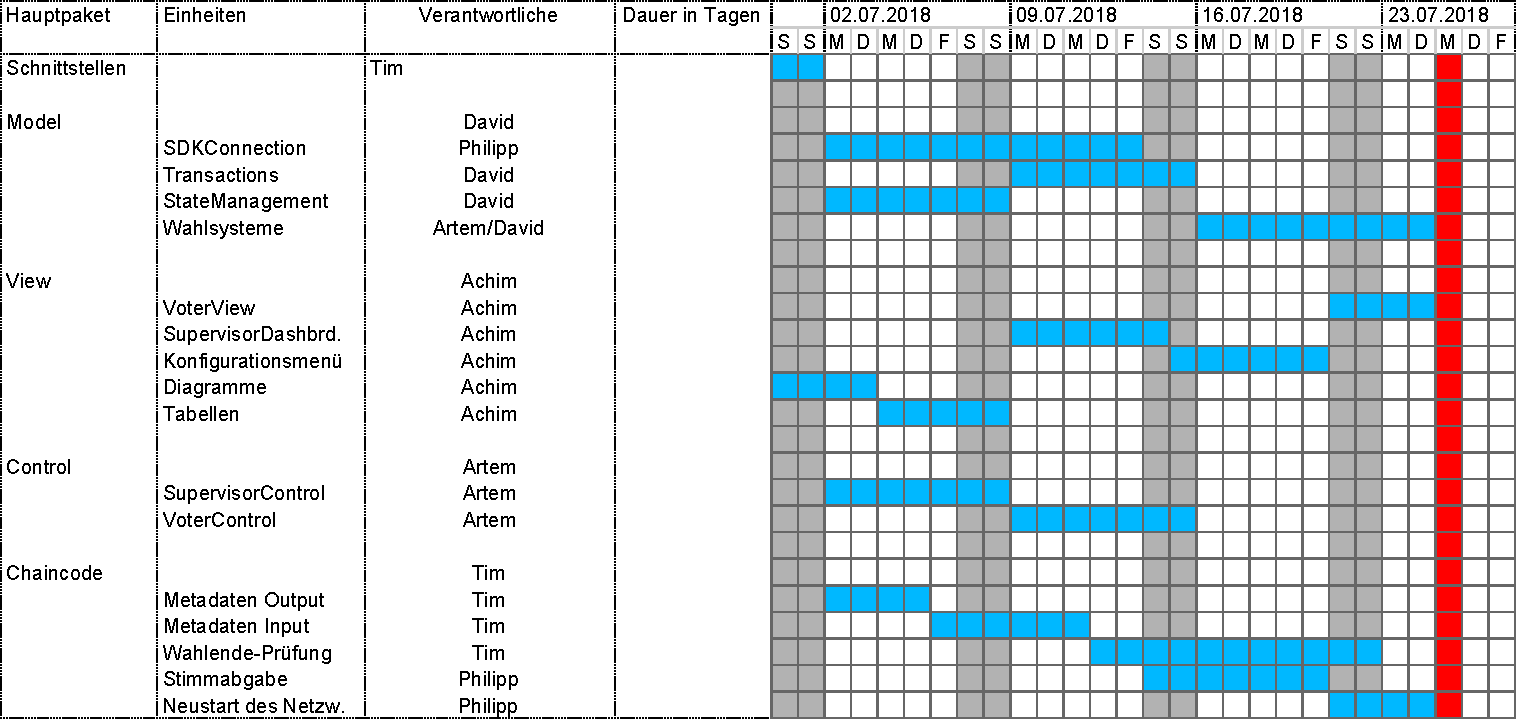
\includegraphics[width=\textwidth]{pictures/Gantt.pdf}
		\caption{Gantt-Diagramm}
		\label{fig:gantt}
	\end{figure}
	\section{Änderung zum Pflichtenheft}
	\subsection{K2: Geheime Wahlen}
	Die Implementierung von geheimen Wahlen zeigte sich bei unseren Nachforschungen als besonders aufwändig, da der Ledger grundsätzlich \enquote{by design} öffentlich ist. Mögliche Strategien wie das Verschlüsseln der Stimmen beim Wähler und späteres Entschlüsseln wurden als Lösung in Betracht gezogen. Selbst hiermit erweist sich die Umsetzung als problematisch, da die Auswertung der Stimmen vom Klienten in die Smart Contracts verlegt werden müsste, um wahrhaft geheim zu sein. Eine solche Auszählung wird durch die verschiedenen Wahlsysteme und deren unterschiedliche Auszählungsverfahren zusätzlich erschwert. Sie wäre in einem solchen System selbst für einen technikaffinen Wähler undurchsichtig, weil nur schwer nachzuverfolgen ist, welcher Chaincode tatsächlich eingesetzt wird. Im Gegensatz dazu könnte beispielsweise der Source Code des Klienten offengelegt werden und ein solcher Wähler könnte nachvollziehen, dass die Auswertung korrekt vonstatten ging. \\ Wir schließen deshalb die Implementierung von geheimen Wahlen nicht aus, bezweifeln aber deren Umsetzbarkeit durch uns. Sollte sich das zu einem späteren Zeitpunkt ändern, ziehen wir sie dennoch in Betracht.

\end{document}
